\chapter{Background}
\label{ch:Background}

In this chapter, we give a broad overview of survival analysis and extend a single end-point survival analysis to a competing risks scenario. We then discuss the two broad classes of approaches used to model competing risks and subsequently motivate the penalized casebase multinomial model. We also include a summary of regularized methods to perform variable selection for competing risks. Finally, we conclude the chapter by discussing the some metrics used to quantify the performance of survival analysis models, which motivate our experiments in Chapter 4. The notation defined in this section is used throughout this work.


\section{Survival Analysis}

We consider a simple multistate model to understand survival analysis, as depicted in \autoref{fig:fig1}. Each individual in the study starts at the initial stage of 0. At some time $T$, the individual moves to the absorbing state 1 which represents the event of interest. Our outcome of interest is this time to event $T$, also known as the survival time. 


\begin{figure}[h]
    \centering
    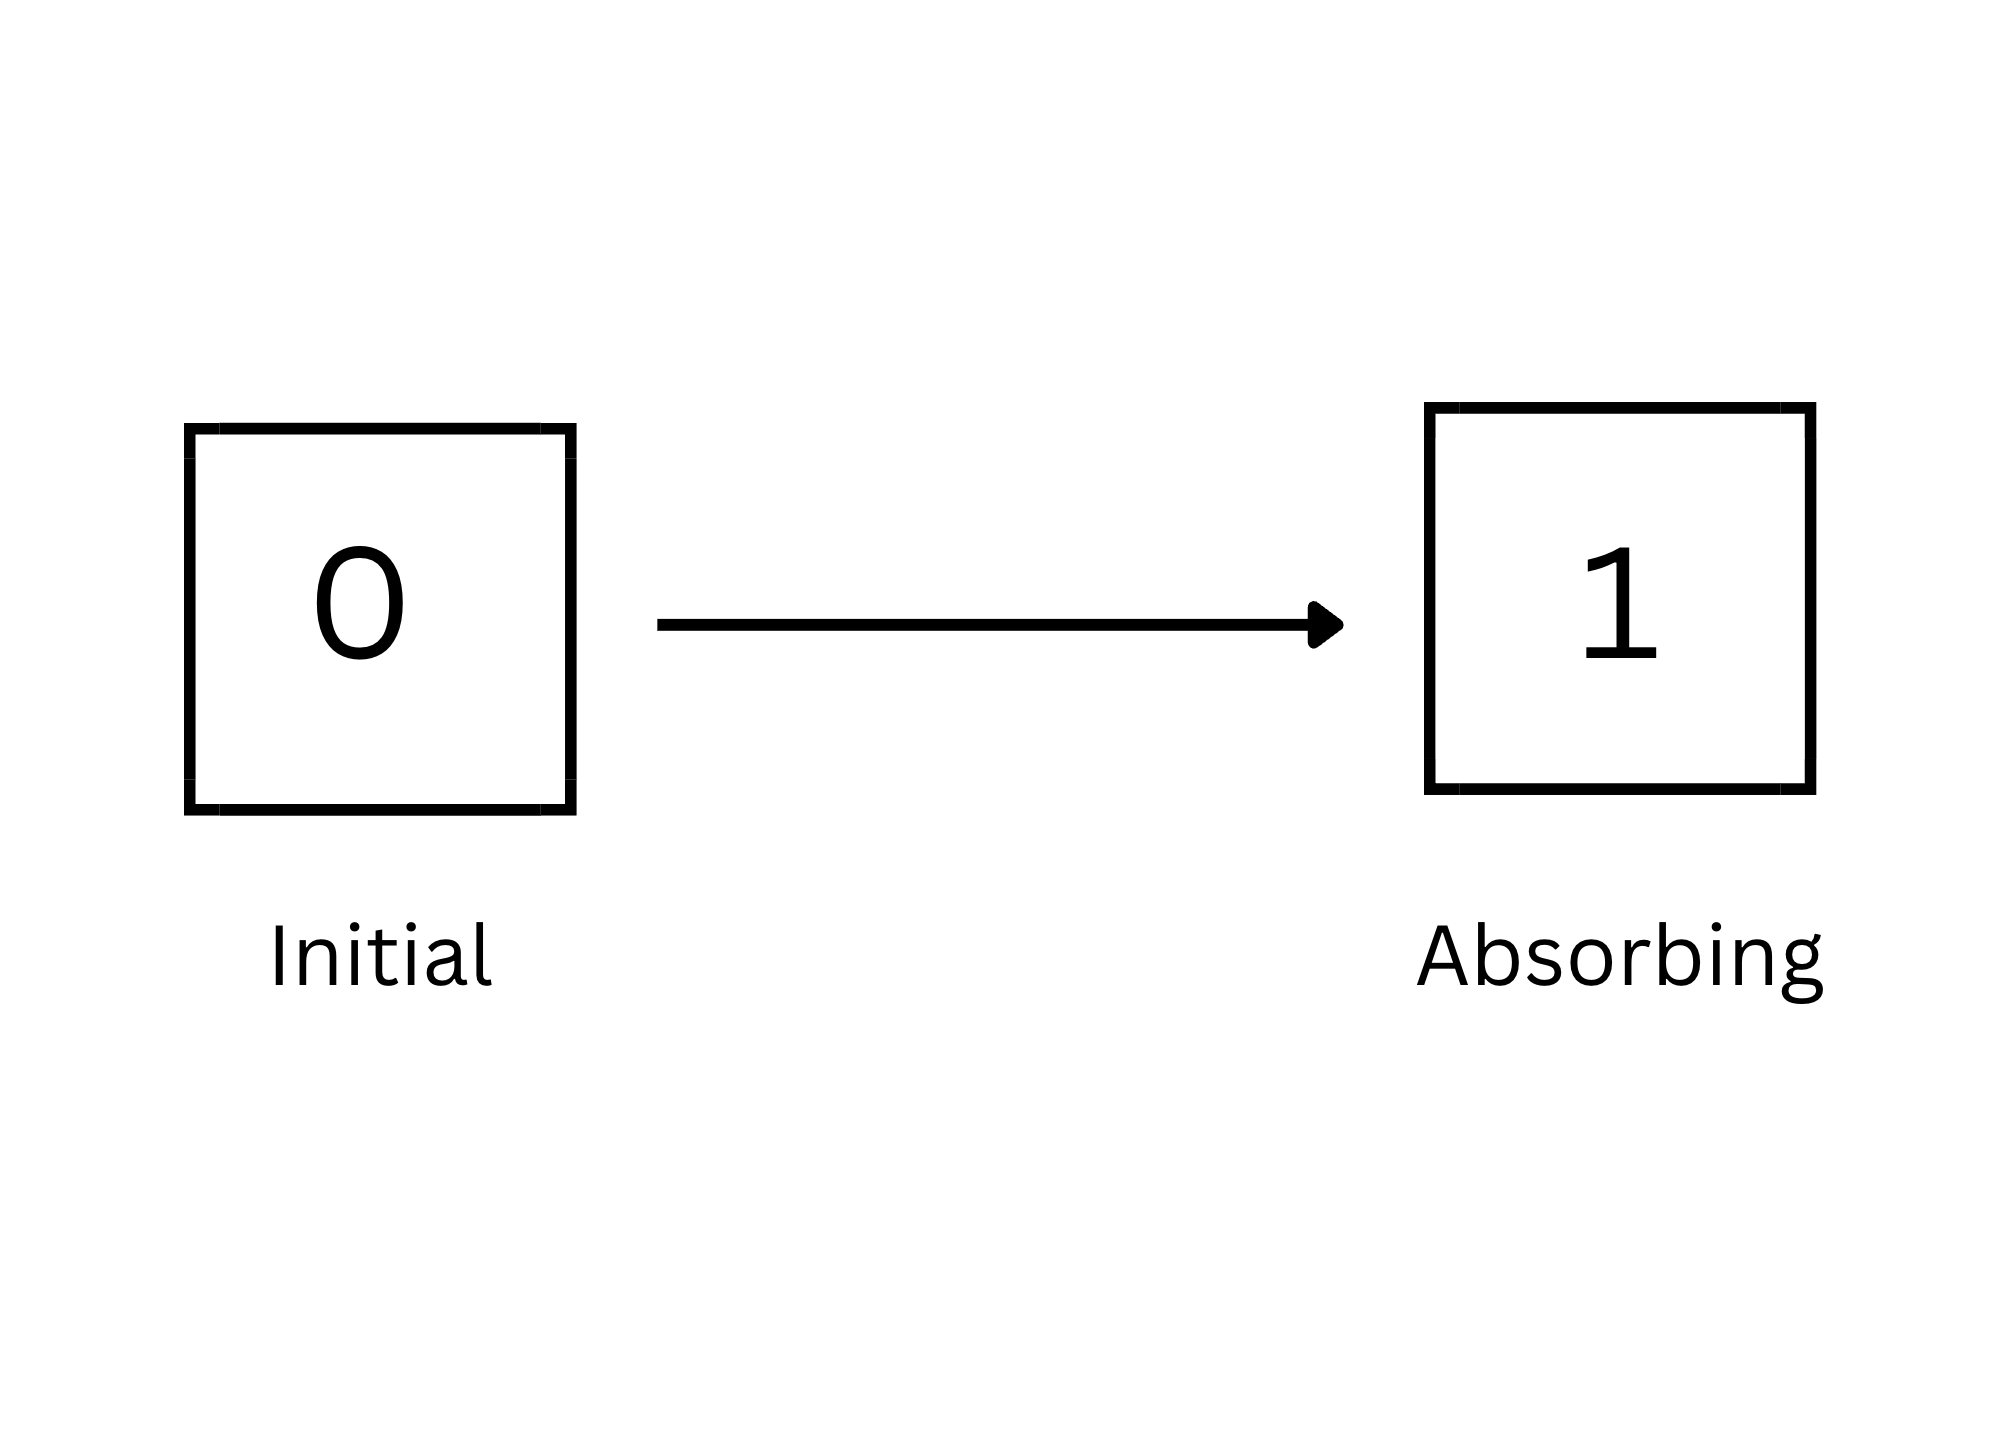
\includegraphics[width=3in]{survival_mstate.png}
    \caption{Single end-point survival analysis represented through a multi-state model}
    \label{fig:fig1}   % label should change
    \end{figure}

In our inference of $T$, we record the state $X_{T}$ at which an individual is at every point of time $t \geq 0$, $X_T \in \{0, 1 \}$. As long as the individual is in the initial stage of 0, they are considered at \textit{risk} to transition to 1. Our time-to event is then the smallest time $T$ at which the individual is no longer in stage 0, i.e. $T := \textrm{inf}\{t : X_{T} \neq 0 \}$. Recording of an individual will stop once the individual has reached the absorbing state 1.
\bigskip \par
Survival analysis has evolved from its initial focus on modeling time to death as the primary event of interest to encompass a wide range of events in various fields of study. Today, it is extensively employed in modeling events such as the time till the onset of disease, time till employment, stock market crashes, earthquakes, and more. In the clinical and biomedical field, time-to-event data remains particularly prevalent and invaluable due to its ability to provide crucial insights into the prognosis and survival outcomes of patients. The development of accurate methods for survival analysis enables researchers and healthcare professionals to effectively assess the effectiveness of interventions and treatments. By incorporating the temporal perspective, survival analysis plays a critical role in understanding the evolving nature of diseases and treatments, allowing for the evaluation of long-term patient outcomes, such as the 5-year risk of disease onset or the probability of patient survival. These insights are essential for guiding clinical decision-making and tailoring treatment strategies to individual patients.
\bigskip \par
Furthermore, survival analysis provides a valuable tool for identifying prognostic factors or covariates that significantly influence survival. By quantifying the effects of specific genetic biomarkers, demographic factors, or treatment modalities, researchers can gain a deeper understanding of the underlying mechanisms that impact disease progression and patient outcomes. This knowledge empowers additionally guides clinical decision-making, as clinicians can further tailor their approach based on the unique characteristics and circumstances of each patient. 
\bigskip \par
In the subsequent sections, we  delve into the details of survival analysis techniques. Additionally, we will discuss how these techniques facilitate the identification of prognostic factors, as well as the quantification of long-term clinical patient outcomes. 

\subsection{Censoring}

A challenging and unique aspect of survival analysis data is censoring. We describe an individual as censored when an observation does not have an exact survival time. There are many reasons that an individual could end up censored in a study, including study drop out, survival up until the end of the study, or for some reason due to which their precise failure time is not observed. 

There are different types of censoring scenarios that could occur, which include left censoring, interval censoring, and right censoring, among which the latter is the most common. Right censoring occurs typically when either 1) an individual experiences the event of interest after the study period, 2) an individual is withdrawn from the study or 3) a subject is lost to follow-up. In this work, we will only consider the scenario of right-censoring, and hence, omit discussion of other censoring schemes. As right-censoring is the most common scheme, there are methods designed specifically for this kind of data, which deal with three categories of right-censored data: Type I, Type II and Type III censoring. 
\smallskip \par
In Type I censoring (which we depict in \autoref{fig:fig2}), we consider the scenario where a study starts with a fixed number of subjects, all of whom have the beginning of the study as the starting point of their observation period. If an individual is lost to follow up, survives till the end of the study, or is withdrawn from the study, their survival time is censored. The survival time is recorded for all other individuals whose time-to-event falls within the study time-period. In this work, we consider Type-I censoring for simplicity and thus, will define the casebase framework under this scenario as well (although it can be extended generally to other censoring scenarios as well). 
\smallskip \par
However, it should be noted that for many survival studies, a common occurrence is Type III censoring, where a study period starts and ends at fixed times, but individuals may enter the study at any time. If we consider two individuals who do not experience the event of interest until the end of the study, unlike Type I censoring, these two individuals will not have the same censoring time, as the two individuals start the study at different times, which needs to be accounted for. 
\smallskip \par
The general takeaway is that censoring complicates the analysis of survival data. The time we actually observe through a survival study can be constructed as $\tilde{T}$ = $(T \wedge C, \textbf{1}(T \leq C))$ i.e the minimum of the event time $T$ and the censoring time $C$. This needs to be addressed carefully by any method proposed for survival analysis.

\begin{figure}[h]
    \centering
    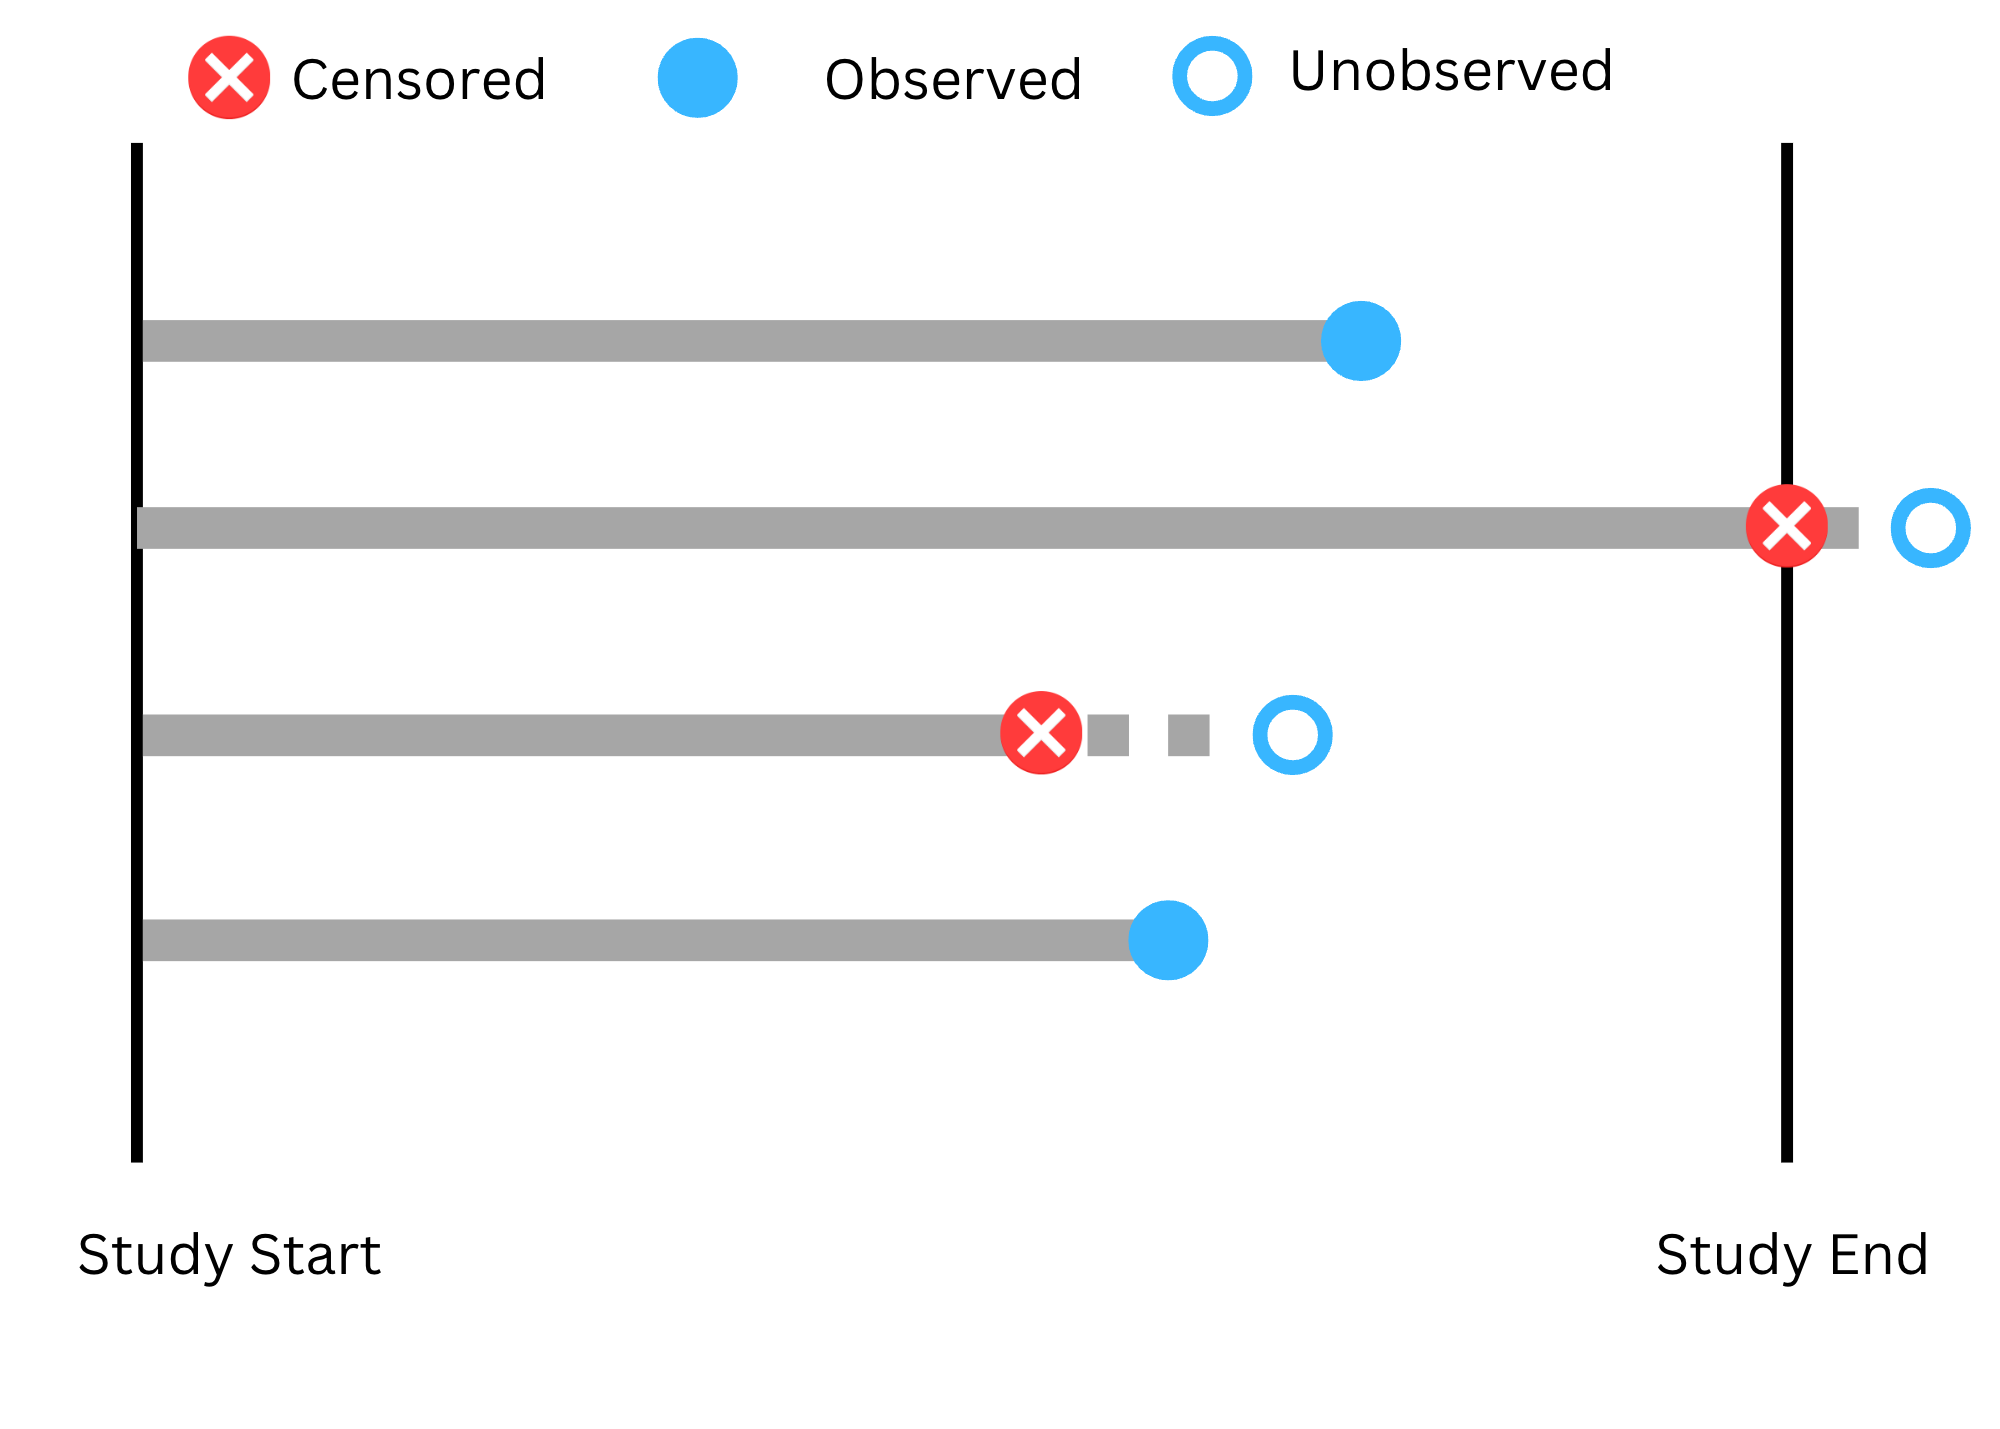
\includegraphics[width=3in]{censoring.png}
    \caption{Schematic of Type I right-censoring. Individual 2 is lost to follow-up and Individual 4 experienced the event after the end of the study, thus both are censored.}
    \label{fig:fig2}   % label should change
    \end{figure}

\subsection{Hazard function}

Typically in a survival analysis, we relate the distribution of $T$ to the covariates of interest by using the hazard function $\alpha(t)$. The hazard can be interpreted as the probability that an individual at risk at time $t$ has an event in time $dt$. Intuitively, the hazard can be interpreted as a rate: specifically the represents the instantaneous event rate for an individual who has already survived to time $t$. The hazard can thus be expressed as: 
\begin{equation}
\alpha(t) \cdot dt := \lim_{\Delta t \searrow 0} \frac{P(T \in [t, t + \Delta t)| T \geq t)}{\Delta t}
\end{equation}

The primary reason that survival analysis methods are hazard-based is due to censoring. As the censoring time $C$ and event $T$ are considered independent, the probability that the event occurs in $dt$ conditional on $T \wedge C \geq t$ is the same as in the absence of censoring, that is:
\begin{equation}
\alpha(t) \cdot dt := \mathbb{P}(T \in dt| T \geq t) = P(T \in dt, T \leq C|T \wedge C \geq t)
\end{equation}

This enables the estimation of the distribution function of $T$ (which we will elaborate on below) even in the presence of censoring, as well as the convenient extension of such hazard-based methods to the competing risks scenario. The intuitive rate interpretation also adds to the advantages of a hazard-based survival analysis approach.

\subsection{The survival function and its relationship to the cumulative hazard}

The distribution function of the event time $T$ can be recovered from the cumulative hazard $A(t)$ as such: 

\begin{equation}
F(t) := 1 - S(t) := P(T \leq t) = 1 - \textrm{exp}(-A(t))
\end{equation}

where $A(t)$ represents the cumulative hazard function $A(t) := \int_{0}^{t} \alpha(u) du$, which provides a measure of the cumulative risk of experiencing an event up to a specific time point. Here, $S(t)$ is referred to as the survival probability. This probability is complementary to the cumulative distribution function $F(t)$, and can be interpreted as the probability that an individual survives longer/is event-free than some specified time \textbf{t}. This probability is often of interest from the perspective of clinical patient care, as the most relevant quantity is often estimating the long-term risk of experiencing a certain event given the patient’s particular characteristics.
\smallskip \par

When analyzing time-to-event data, The Kaplan-Meier estimator is a commonly used non-parametric method for estimating the survival function $S(t)$.
Through this estimator, the survival function can be expressed as a product integral of the cumulative hazards over time $t$ as such: 
\begin{equation}
S(t) = \Prodi_{0}^{t} (1- d\hat{A}(u)) \approx \prod_{k = 1}^{K} (1- \Delta \hat{A}(t_k)) \approx \prod_{k = 1}^{K} P(T > t_k | T > t_{k-1})
\end{equation}

where the ordered sequence of observed event times $0 = t_0 < t_1 < t_2 <...< t_{K-1} <t_K$ partitions the time interval $[0,t]$. The cumulative hazard $\hat{A}(t_k)$ is represented by the Nelson-Aalen estimator here, which can be written as:
\begin{equation}
\hat{A}(t_k) = \frac{\text{Number of individuals \textit{observed} to fail at $t_k$}}{\text{Number of individuals \textit{at risk} just prior to $t_k$}}
\end{equation}


The Kaplan-Meier estimator provides a stepwise estimate of the survival function by taking into account the observed event times and censoring information. The Nelson-Aalen estimator is also non-parametric method, which estimates the cumulative hazard function $A(t)$ directly from the observed event times. It takes into account both the observed events and the associated event times, without assuming any specific distribution for the hazard function. Both the Kaplan-Meier estimator and the Nelson-Aalen estimator are valuable tools in a single-end point survival analysis, allowing researchers to estimate the survival function and the cumulative hazard function, respectively. These estimators provide valuable clinical insights into the survival experience and cumulative risk of experiencing an event over time, even in the presence of censored data. It is important to note the connection back to the hazard function here, namely that the accurate estimation of the cumulative hazard plays an essential role in estimating the survival function.


\section{Cox-Proportional Hazards Model}

Survival analysis has been greatly shaped over the last few decades by the partial likelihood approach of the Cox proportional hazard model. The Cox Proportional Hazards model specifies that the conditional hazard function of failure time given a set of covariates is the product of an unknown baseline hazard function and an exponential regression function of covariates of the form:
\begin{equation}
\lambda(t|X_i) = e^{\beta^T X_i(t)} \lambda_0 (t)
\end{equation}

Here, $X_i = (X_{i1}, … , X_{ip})$ represent the realized values of the covariates for subject $i$, $\lambda(t|X_i)$ represents the  hazard function at time $t$ for subject $i$ with covariate vector $X_i$, $\beta$ represents an unknown set of regression parameters. 
\smallskip\par
Note that the baseline hazard between subjects is identical ($\lambda_0 (t)$) with no dependency on $i$. This is connected to the "proportional" aspect of the Cox model, i.e. its assumption that the hazards for any two individuals have the same proportion at all times, which can be shown as below:
\begin{equation}
\frac{\lambda(t|X_2)}{\lambda(t|X_2)} = \frac{\lambda_0 (t) \dot e^{\beta_2^T X_1(t)}}{\lambda_0 (t) \dot e^{\beta_1^T X_2(t)}} = \frac{e^{\beta_2^T X_1(t)}}{e^{\beta_1^T X_2(t)}}
\end{equation}

i.e the only difference between subjects' hazards comes from the baseline scaling factor $e^{\beta^T X_i(t)}$. In a Cox proportional hazards regression model, the measure in relation to which the regression coefficients are quantified is the hazard rate. In etiological studies, it is often of interest to assess the association between several risk factors and survival time, and interpretation in terms of the hazard is often ideal for this type of analysis. For example, we can easily make interpretations such as a 1-unit change in Age can increase the rate of occurrence of event by 2.11 with the coefficients estimated by a Cox-Proportional Hazards model. The hazard ratios estimated by the Cox model are among those individuals who are actually at risk of developing the event of interest i.e. ‘among those patients who did not (yet) experience the event of interest or a competing event’. As such, this hazard-based modelling approach has the advantage of being easily interpretable for clinicians in studies where the aim of interest is to quantify the effect of prognostic risk factors/covariates in relation to survival time for the \textit{risk set} of patients. 
\smallskip\par
Note that in the estimation of a Cox Proportional Hazards model, the baseline hazard $\lambda_0 (t)$ is treated as a nuisance parameter, and is not estimated with the coefficients. Thus, the cumulative baseline-hazard function needs to be separately estimated. However, the cumulative baseline-hazard is an essential quantity to estimate the survival function. To this end, the Breslow estimator, which extends the Nelson-Aalen estimator to the Cox model with coefficients was proposed to estimate the baseline cumulative hazard function for a Cox model, which takes the form: 
\begin{equation}
\hat{A}_0(t) = \sum_{i =1}^{n} \frac{I(\tilde{T_i} \leq t) \Delta_i}{\sum_{i \in \mathcal{R}_i} \exp(\hat{\beta}^T \mathbf{X}_i(\tilde{T_i}))}
\end{equation}

where  $\tilde{T}$ = $(T \wedge C, \textbf{1}(T \leq C))$, $I(.)$ represents the indicator function, and $\Delta_i$ represents the numerator of the Nelson-Aalen estimator, i.e the number of individuals \textit{observed} to fail at $t$. The conditional survival function under $X = x$ can then be estimated from the Cox model as such:
\begin{equation}
\hat{S}(t) = \exp \left\{ - \int_{0}^{t} exp(\hat{\beta}^T x(u)) d\hat{A}(u) \right\}
\end{equation}

The conditional survival survival function with the Breslow estimator provides a more accurate approximation than the Kaplan-Meier estimator by assigning equal weight to all individuals at risk within each interval. The Breslow estimator comes with the advantage of being non-parametric and not assuming a specific form for the hazard, as its estimation process is based on summing up the number of events at each time-point. However, this comes at a cost of estimating a step-wise survival function (depicted in \autoref{fig:fig3}). As a result of the estimation process, the step-wise Breslow estimate exhibits sudden changes or jumps at the observed event times. These jumps can make it challenging to visually interpret the estimated survival function, especially in small samples, when there are a limited number of observed event times or when the event times are irregularly spaced. The jumps in the estimated survival function can give the impression of abrupt changes in survival probabilities, even when the underlying true survival function may exhibit a smoother and more gradual change over time, and thus, can be difficult to interpret. Estimating the survival function for a patient is more convenient and interpretable through a parametric formulation for this reason. 

We note that although Breslow (1972) did suggest a smoothed estimation of the baseline hazard function, this is not available in most of the popular survival analysis software packages, as the step-wise estimator can be derived with more ease relatively. Additionally, while parametric extensions to the Cox Regression model have been proposed, such as the Weibull-Cox, the use of such models would require 1) the assumption of a parametric family which negates the benefits of the semi-parametric formulation of the Cox-regression model and 2) an understanding of how the changes in the covariates affect the Weibull distribution's shape and scale parameters, which can be challenging to interpret for the clinician. 

\begin{figure}[h]
    \centering
    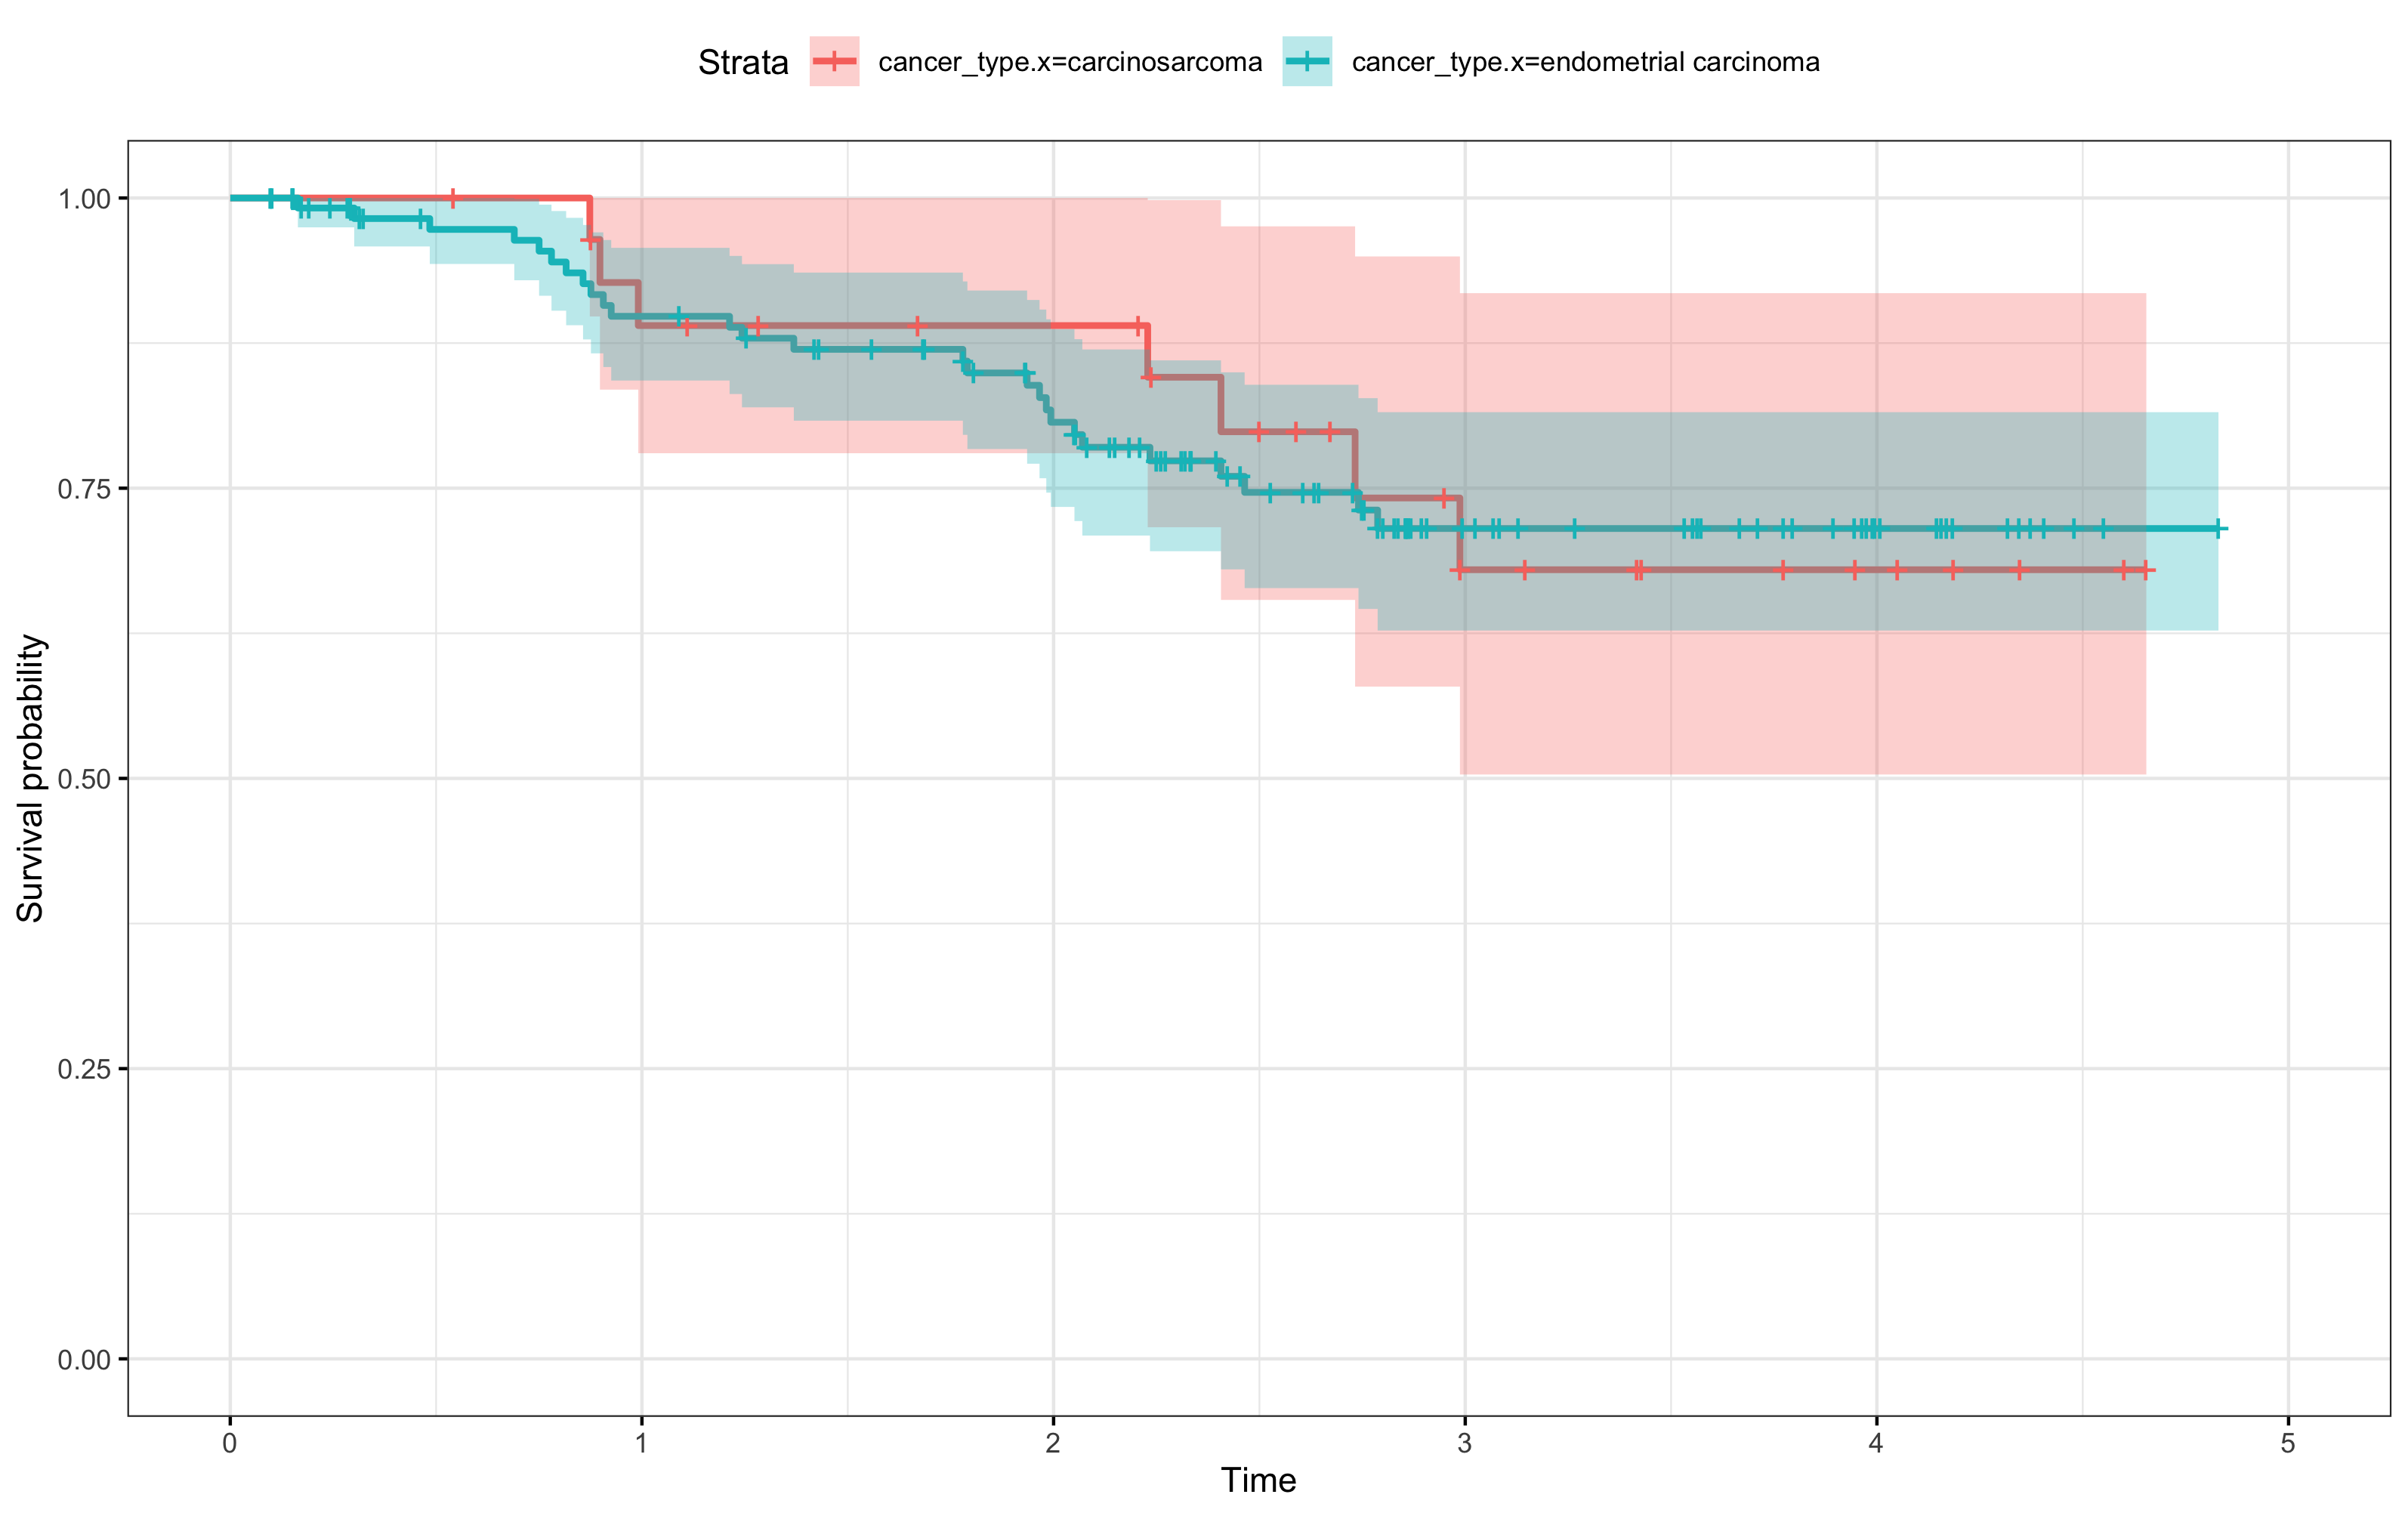
\includegraphics[width=3in]{cancertype.png}
    \caption{Step-wise survival curves estimated by the Breslow Estimator}
    \label{fig:fig3}   % label should change
    \end{figure}


\section{Competing Risks}

Understanding competing risks is now relatively intuitive as an extension of  the single-endpoint framework in terms of a multi-state model. A general survival model can be generalized to a competing risks setting by introducing several competing absorbing states, which represent the possible event types. In this setting, we can model the occurrence of a competing event as a transition into the corresponding competing event state. This model is depicted in \autoref{fig:fig4} for a finite number ($J$) competing risks. While this is theoretically possible under the competing risks framework, we only consider the simplest case ($J = 2$) in this work, which is also the most commonly collected type of competing risks data.


\begin{figure}[h]
    \centering
    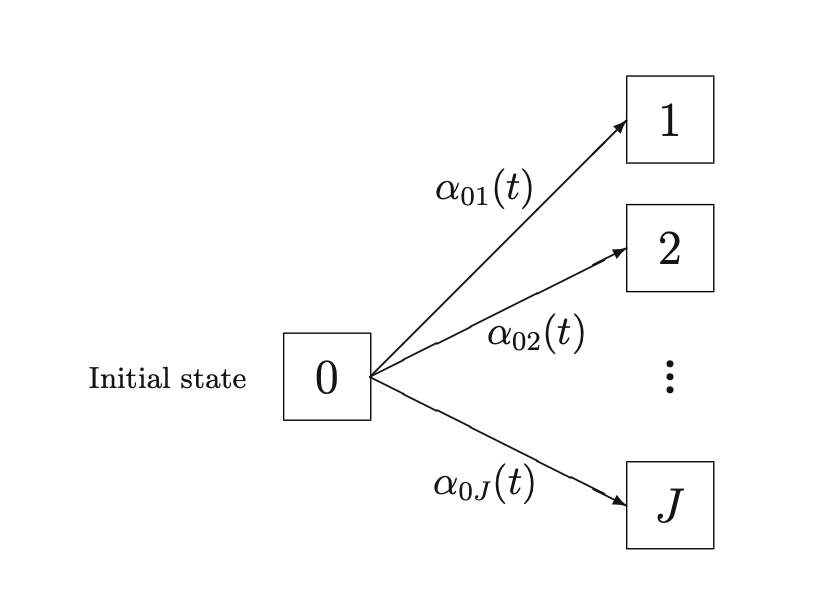
\includegraphics[width=3in]{competing_risks.png}
    \caption{Competing risks multistate model with cause-specific hazards $\alpha_{0j}(t), j = 1, 2, ....., J$. The vertical dots The vertical dots indicate the competing event states 
    $3, 4, ...., J-1$.}
    \label{fig:fig4}   % label should change
    \end{figure}

\begin{figure}[h]
    \centering
    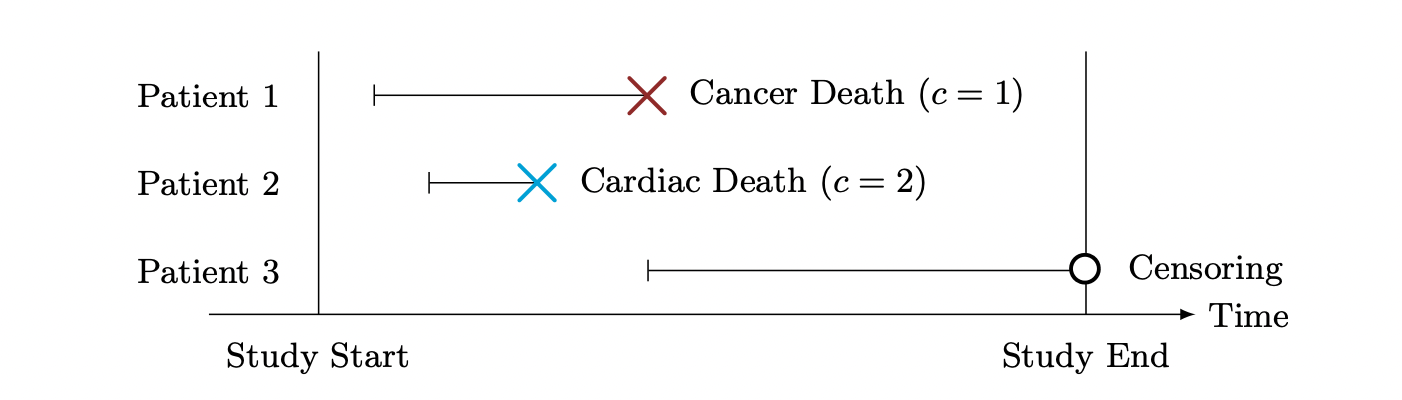
\includegraphics[width=6in]{competingrisks_example.png}
    \caption{Schematic of observation times for three example patients with competing risks}
    \label{fig:fig6}   % label should change
    \end{figure}

To look at an example (\autoref{fig:fig6}), when studying the survival of cancer patients, competing events can be cancer-related death $(c = 1)$, our primary cause of interest, or death by cardiac disease $(c = 2)$. An individual is no longer \textit{at risk} of cardiac disease once they have died of cancer, and vice versa, i.e they are mutually exclusive events.
We can use single end-point survival analysis, such as the Kaplan-Meier estimate to analyze competing risks data and estimate the survival function by recording other events as censored observations. However, the independent censoring assumption $(T \wedge C)$ does not hold in this setting: it may be unreasonable to assume that subjects who died of the competing risk (and were thus treated as censored) can be represented by those subjects who remained alive and had not yet died of any cause.  This can lead to biased estimates in standard survival models, as well as overestimation of the survival function.
\smallskip \par 
In recent years, the analysis of competing risks data has gained increasing prominence in various fields of study, but yet remains an area of survival analysis that has been relatively less-explored. As populations age and chronic diseases become more prevalent, the occurrence of multiple competing events, such as multiple types of diseases or comorbidities, has become a critical aspect of research. The availability of large-scale longitudinal datasets has facilitated need for the accurate analysis of competing risks. Thus, understanding and appropriately analyzing competing risks data is essential for accurate risk assessment, for identifying prognostic factors and for clinical decision-making, to accurately account for patients being \textit{at risk} for more than one comorbidity.

\subsection{Cause-specific Hazards}

Under competing risks, the hazard function translates to cause-specific hazards $\alpha_{0j}(t), j = 1, 2$, one for each event in a two-competing risks setting, of the form: 
\begin{equation}
A_{0j}(t) := \int_{0}^{t} \alpha_{0j} (u) du, j = 1, 2
\end{equation}

In a competing risks analysis, both cause-specific hazards (which can be thought of as "transition intensities") completely determine the stochastic behaviour of the competing risks process in the multistate model.

\subsection{Cumulative Incidence Function (CIF)}

As previously discussed, from the perspective of clinical patient care, the most relevant quantity is often estimating the long-term risk of experiencing a certain event given the patient’s particular characteristics. This is often of interest in the competing setting, and is captured by estimating the cumulative incidence function (CIF) or the absolute risk, i.e., the expected proportion of individuals experiencing a certain event over the course of time. The cumulative incidence function for each cause can be expressed as function of the cause-specific hazards and the survival function $P(T > u-)$ as shown below: 

\begin{equation}
    P(T \leq t) = \int^{t}_{0} P(T > u-) \alpha (u) du
\end{equation}

The cumulative incidence function was proposed to solve the inadequacy of the Kaplan-Meier estimate for competing risks data by estimating the marginal probability of an event of interest as a function of its cause-specific hazard and the overall survival probability. In the simple single-endpoint survival analysis setting, it breaks down to $1- \hat{S}(t)$, where $\hat{S}(t)$ is the Kaplan Meier estimate. 

\section{Regularization and Variable Selection for Survival Analysis}

TALK ABOUT HIGH-DIMENSIONAL DATASETS, NEED TO PREVENT OVERFITTING, IDENTIFY IMPORTANT GENES/BIOMARKERS

OVERVIEW OF ELASTIC NET FAMILY: FOCUS ON LASSO

\section{Regularized modelling approaches for competing risks}

TALK ABOUT CAUSE-SPECIFIC AND CIF MODELS DIFFERENCE 

MODELS TO TALK ABOUT: 

1) BOOSTED COX
2) PENALIZED FINE-GRAY
3) PENALIZED COX
4) DIRECT BINOMIAL

\section{Survival Analysis Model Performance Measures}

1) BRIER SCORE

2) TALK ABOUT SENS, SPEC, MCC
